\chapter{Introducción}\label{cap.introduccion}
En este capítulo se situará el Trabajo Fin de Máster en el marco existente en la actualidad, explicando el campo que comprende la \acrfull{va}, las \acrfull{rna} y la tarea de predicción. Además se exponen los objetivos a alcanzar en el desarrollo del trabajo y la metodología empleada para ello.

\section{Visión artificial}

Desde que apareció el primer ordenador en el planeta, el ser humano ha soñado con que estas máquinas puedan realizar tareas humanas, incluyendo su capacidad de pensar y tomar decisiones. Algunos de los ejemplos de estas tareas, propiamente humanas, se encuentran en el reconocimiento del habla, el entendimiento de las imágenes o la automatización de procesos. El campo de estudio que trata estos aspectos y se focaliza en el aprendizaje de las máquinas es la denominada  \acrfull{ia}\cite{Goodfellow-et-al-2016}, cuya presencia es cada vez mayor en la vida cotidiana.\\

Hoy en día el campo de la \acrshort{ia} abarca muchas de las tareas que antes requerían de la acción humana; sin embargo, los resultados que pueden alcanzar los algoritmos en las máquinas no es siempre suficiente. A pesar de que la capacidad de cómputo que tienen algunas máquinas es mucho mayor que la del ser humano, aún no se les ha logrado dotar de otros aspectos importantes como la empatía o las emociones. Este hecho hace que la actividad del cerebro humano siga siendo necesaria en muchas de las situaciones a las que se pueden enfrentar las personas.\\

La \acrshort{ia} se aplica en la solución de problemas como la identificación biométrica, el diagnóstico de enfermedades, los estudios de mercado o la robótica. Este campo hace, hoy en día, uso de desarrollos en el ámbito del \textit{Machine Learning}, las \acrshort{rna}, el procesamiento del lenguaje natural, el procesamiento del habla o la \acrshort{va}, donde se pone el foco de este trabajo. Todas estas alternativas de desarrollo no se presentan de forma única, sino que las soluciones suelen aplicar varias de ellas, complementadas entre sí, para abordar distintos problemas. \\

La \acrfull{va} es la disciplina que permite a las máquinas entender el mundo físico a través del procesamiento de las imágenes. Su objetivo es emular la actividad de los ojos y el cerebro del ser humano para explorar el mundo real, actuando en consecuencia con lo procesado. Este campo presenta distintas alternativas y se ve influido por distintas áreas afines que aportan distintos conceptos a la disciplina, representadas en la Figura~\ref{fig.vision}. Las áreas representadas en color azul aportan distintos valores a la disciplina, y son necesarias para su buen funcionamiento. Áreas como las matemáticas o la física ayudan a la comprensión del mundo real, mientras que otras, como la técnica de imagen, ayudan a la adquisición de datos.

\vspace{20pt}
\begin{figure}[H]
		\begin{center}
			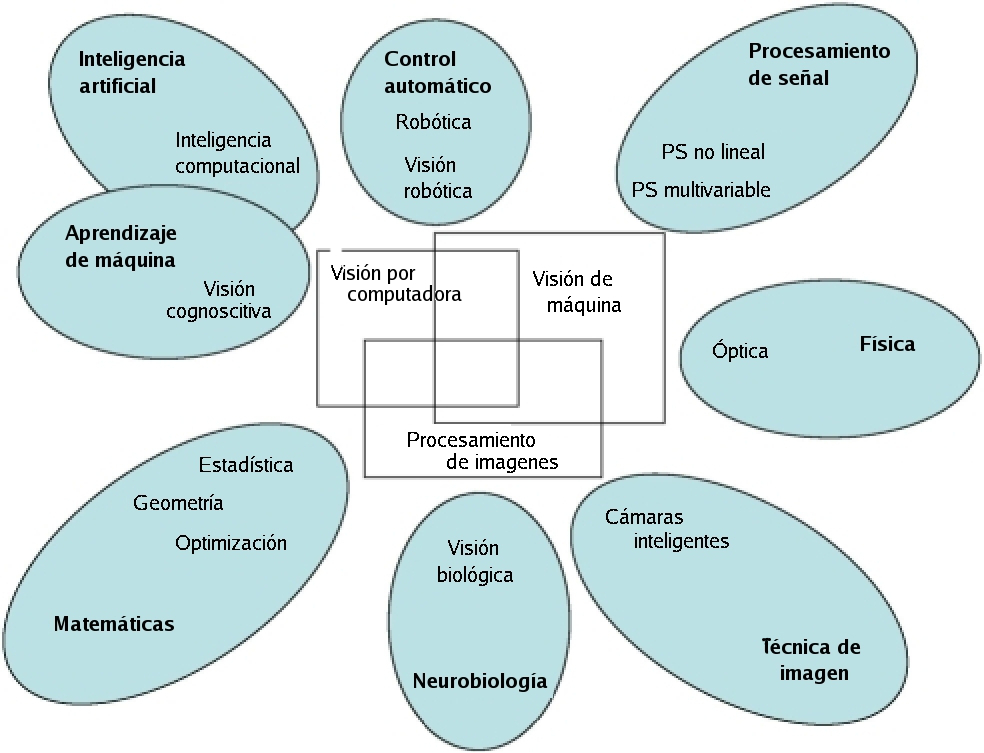
\includegraphics[width=0.7\textwidth]{figures/intro/vision.jpg}
			\caption{Esquema de las relaciones entre la \acrshort{va} y otras áreas. Gráfico obtenido de~\cite{vision}.}
			\label{fig.vision}
		\end{center}
\end{figure}
\vspace{-10pt}



La \acrshort{va} tiene aplicaciones muy diversas en campos tan distintos como la medicina y la fabricación industrial. Además, en los últimos meses ha jugado un papel muy importante durante la pandemia del COVID-19 con soluciones que han permitido realizar controles de aforo, identificación a distancia o toma de temperatura sin contacto.\\

Uno de los ejemplos de aplicación más extendidos es el uso de algoritmos sobre imágenes de naturaleza médica (TACs, radiografías, ecografías...) como sistemas de ayuda al diagnóstico de enfermedades como el cáncer, mostrado en la Figura~\ref{fig.tumor}. La empresa Microsoft está desarrollando su propio proyecto de investigación, \textit{InnerEye}~\cite{innereye}, cuyo objetivo radica, precisamente, en facilitar el diagnóstico proporcionando mayor precisión en el mismo y la posibilidad de combinar la imagen con otro tipo de datos que complementen la información extraída a través de imagen médica.

\begin{figure}[H]
		\begin{center}
			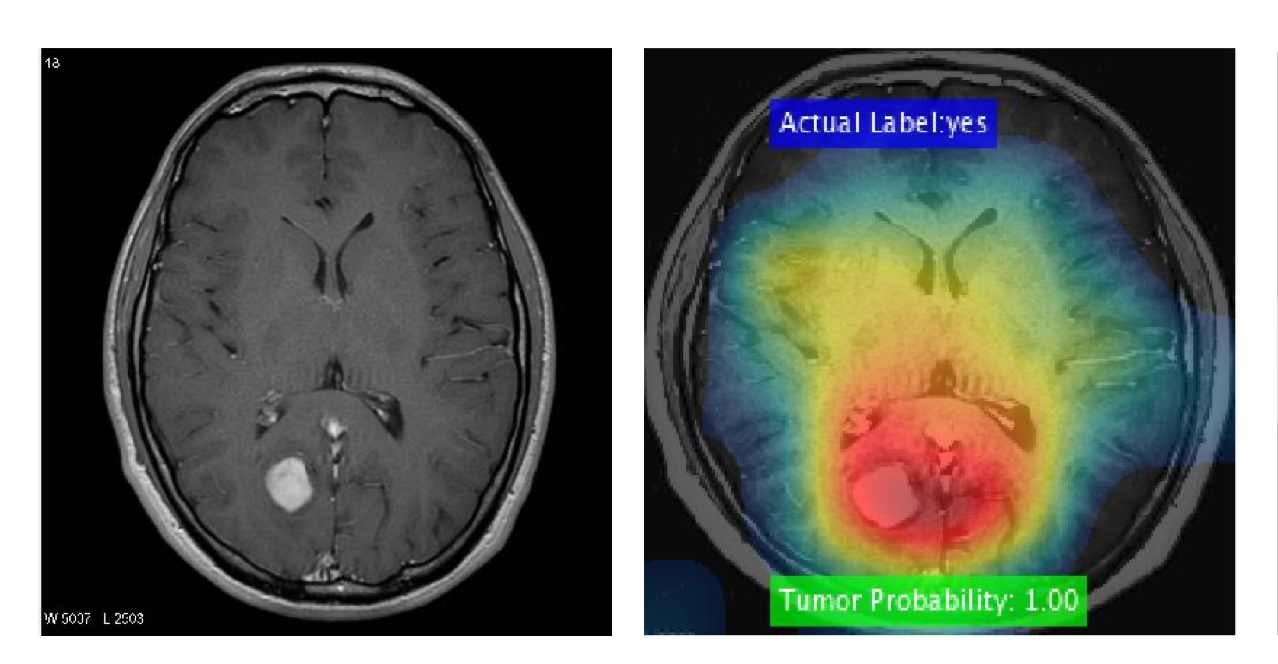
\includegraphics[width=0.7\textwidth]{ figures/intro/tumor.png}
			\caption{Detección de tumores cerebrales mediante \acrshort{va}. Imagen obtenida de~\cite{narayanan2019understanding}.}
			\label{fig.tumor}
		\end{center}
\end{figure}
\vspace{-10pt}

Otro ejemplo de aplicación de la \acrshort{va}, esta vez en el mundo de la biometría, consiste en facilitar la identificación de las personas de forma remota. Mediante la extracción de la información de un documento de identidad y la petición de fotografías o vídeos al usuario, se desarrollan los llamados sistemas de \textit{onboarding} (véase la Figura~\ref{fig.onboarding}). Estos sistemas facilitan el proceso de alta en determinados productos, como una cuenta bancaria, o plataformas, como una casa de apuestas, que por su naturaleza necesitan de una identificación veraz. Durante los últimos meses, este sistema ha experimentado un gran impulso en su uso ya que facilita no tener contacto interpersonal, un factor determinante para frenar la expansión del COVID-19.

\begin{figure}[H]
		\begin{center}
			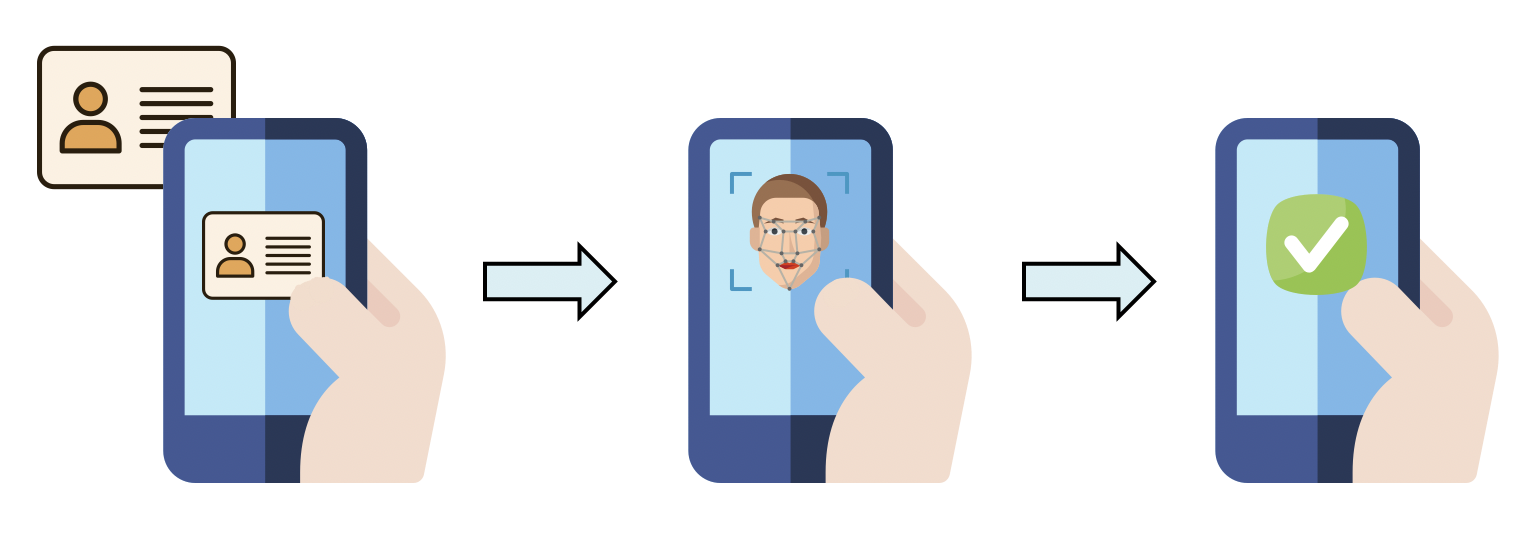
\includegraphics[width=0.6\textwidth]{ figures/intro/onboarding.png}
			\caption{Flujo de una aplicación \textit{onboarding}.}
			\label{fig.onboarding}
		\end{center}
\end{figure}
\vspace{-10pt}

Un último ejemplo de aplicación de la \acrshort{va} se encuentra en la detección de personas u objetos. Esta tarea no se suele realizar de forma independiente, sino que se aúna con otras como el conteo o el seguimiento. En relación a la primera, el conteo de personas, si bien es una tarea bastante sencilla tras la detección, ha tomado un alto grado de importancia en los últimos meses. La necesidad de control de aforo en lugares abiertos, como las playas~(véase Figura~\ref{fig.aforo}), y cerrados, como los aeropuertos, ha impulsado la presencia de estas tecnologías de \acrshort{va} en el día a día.
\vspace{10pt}
\begin{figure}[H]
		\begin{center}
			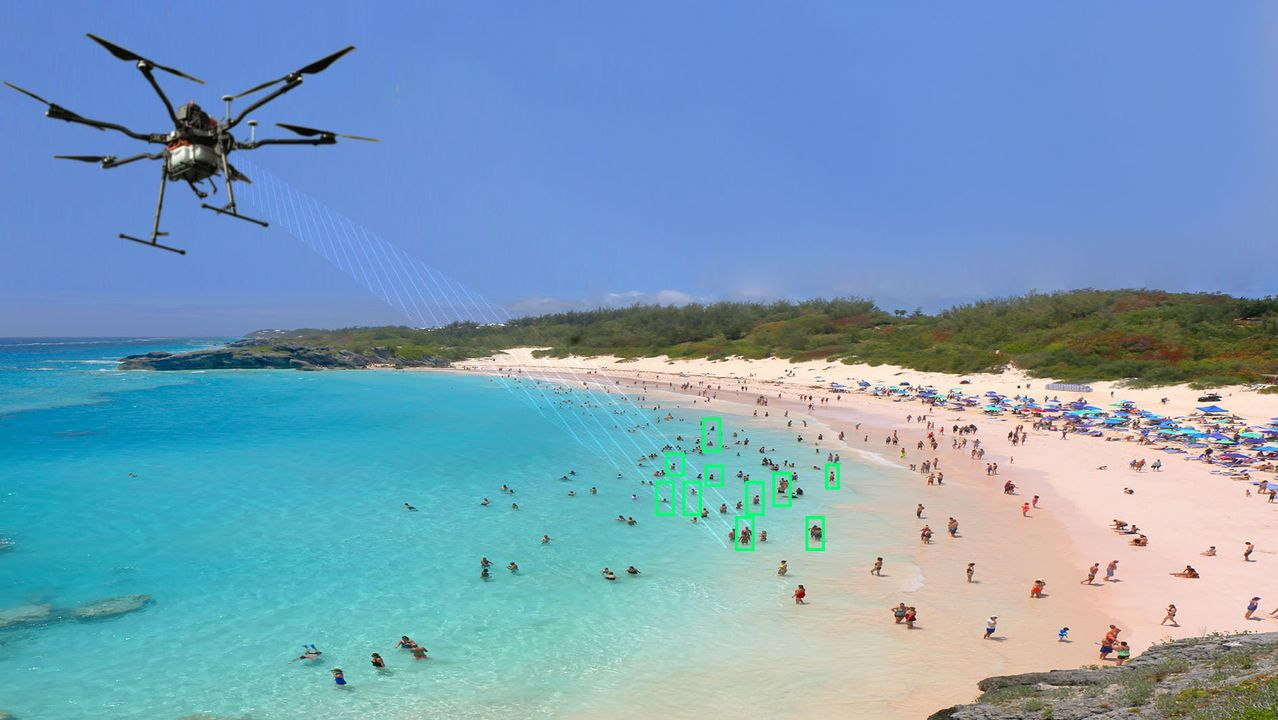
\includegraphics[width=0.75\textwidth]{ figures/intro/aforo.jpg}
			\caption{Control con drones del aforo en las playas mediante \acrshort{va}. Imagen obtenida de~\cite{aerocovid}.}
			\label{fig.aforo}
		\end{center}
\end{figure}
\vspace{-10pt}

En cuanto al seguimiento, tras detectar a la persona en imágenes sucesivas es posible establecer la trayectoria que ésta ha seguido, según se muestra en la Figura~\ref{fig.track}. En este caso es posible introducir la predicción en una secuencia de imágenes, tema sobre el que versa este trabajo, como una solución a las pérdidas del objeto, es decir, los momentos en los que el objeto que estaba siendo seguido por una máquina no logra ser detectado por la misma. Cuando el sistema no detecta el objeto, por ejemplo por una oclusión, el sistema puede realizar una estimación de la posición en la que el objeto puede aparecer en instantes sucesivos. Ello permite reducir la zona de una nueva búsqueda para volver a detectar el objeto y dar continuidad al seguimiento.
\vspace{10pt}
\begin{figure}[H]
		\begin{center}
			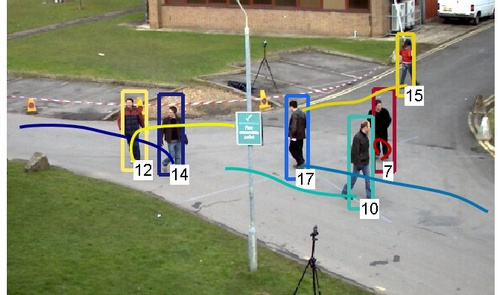
\includegraphics[width=0.75\textwidth]{ figures/intro/tracking.jpg}
			\caption{Seguimiento de personas con \acrshort{va}. Imagen obtenida de~\cite{tracking}.}
			\label{fig.track}
		\end{center}
\end{figure}

\section{Redes neuronales artificiales}
El aprendizaje máquina, \textit{Machibe Learning}, se utiliza en muchos campos, incluyendo la \acrshort{va}. El proceso de aprendizaje de las máquinas puede realizarse de forma supervisada o no supervisada. Si cuando se proporcionan las muestras al algoritmo para que aprenda, además de las características, se le proporciona una etiqueta que indica la salida deseada del algoritmo, se está ante un proceso supervisado. Si, por el contrario, la única entrada que alimenta el algoritmo son las características crudas, el algoritmo de aprendizaje se considera no supervisado. Los algoritmos de aprendizaje supervisado abordan tareas de clasificación y estimación, cuyo principal objetivo es encontrar la función que mapea entradas con salidas. Por otro lado, los algoritmos no supervisados abordan tareas de agrupamiento, creando grupos de ejemplos con características similares entre sí y distintas a las del resto.\\

Una de las ramas de aprendizaje máquina más exitosas en los últimos años es la del aprendizaje profundo, que maneja \acrfull{rna}. Las \acrshort{rna}\cite{rna} son modelos matemáticos que tratan de emular el funcionamiento del cerebro humano mediante la interconexión de neuronas distribuidas en varias capas. El objetivo principal de estos modelos es conseguir que las máquinas sean capaces de aprender a través de su entrenamiento con un conjunto de datos. Gracias al entrenamiento se consigue que estas redes puedan ofrecer resultados satisfactorios cuando se les presenta un ejemplo que no han visto antes, lo que indica que la red ofrece buena capacidad de generalización.\\

El proceso de entrenamiento o aprendizaje de las \acrshort{rna}, proceso en el que se fijan los pesos de las distintas conexiones entre las neuronas de cada capa, se afronta como un problema de minimización de una función de coste o función de \textit{loss}. Para ajustar los  pesos de la red se emplea la propagación del error ``hacia atrás'' haciendo uso de un método de cálculo del gradiente una vez la red se ha inicializo con una serie de pesos. Al introducir un ejemplo en la estructura, éste se propaga desde la primera capa a las sucesivas hasta generar una salida. Esta salida se compara con la salida deseada y se obtiene un error, que es trasladado desde la capa de salida hasta la de entrada, permitiendo el ajuste de los pesos en consecuencia. Es decir, se puede ver el entrenamiento como una aplicación directa de la teoría de optimización.\\

Existen redes monocapa, compuestas por una única capa en la que las neuronas crean conexiones laterales para conectarse entre ellas en la propia capa, como la red de Hopfield. Sin embargo, en este trabajo se utilizan las redes multicapa, compuestas por múltiples capas conectadas entre sí. Cuando se trabaja con varias capas, éstas se clasificadas en tres tipos:
\begin{itemize}
    \item \textbf{Capa de entrada:} Formada por las neuronas que introducen los datos a la red.
    \item \textbf{Capas ocultas:} Las capas intermedias, que realizan diferentes transformaciones. Las transformaciones que realizan estas capas, no tienen por qué coincidir dentro de una misma red.
    \item \textbf{Capa de salida:} Constituida por las neuronas que se corresponden con la salida. 
\end{itemize}


La introducción del aprendizaje profundo, con las \acrshort{rna}, en el mundo de la \acrshort{va} ha supuesto una gran revolución, comenzada en el año 2012. Las \acrshort{rna} han permitido descubrir relaciones no lineales que no era posible captar con los algoritmos tradicionales. Las \acrshort{rna} han introducido un alto grado de mejora en las aplicaciones utilizan las técnicas de \acrshort{va} tradicional, como los filtros de \textit{Kalman}. Se consigue un incremento en la calidad de las aplicaciones sustituyendo, además, un gran esfuerzo humano para la obtención de descriptores por un procesamiento de máquina mucho más rápido y eficaz. Otro factor que hace de las \acrshort{rna} una buena alternativa a las técnicas tradicionales es que el ajuste de una aplicación en un entorno nuevo no suele conllevar un desarrollo muy complejo, se puede conseguir una buena adaptación con un nuevo reentrenamiento específico.\\

El aprendizaje profundo ha sido aplicado con éxito en una gran variedad de problemáticas, de distinta naturaleza, favoreciendo su alto grado de implementación en la actualidad. Un ejemplo de aplicación de \acrshort{rna}, en un contexto distinto a la \acrshort{va}, es reconocimiento del lenguaje. Aplicaciones como \textit{Siri} o \textit{Alexa} hacen uso de esta tecnología para ``escuchar'' al ser humano y realizar acciones como poner una canción o llamar a una persona.\\

Dentro de la \acrshort{va} un ejemplo de la implementación de las \acrshort{rna} en la tarea de clasificación es la conocida como \textit{AlexNet}~\cite{NIPS2012_4824}, cuyo ejemplo de aplicación se muestra en la Figura~\ref{fig.alexnet}. Esta red fue desarrollada con el objetivo de clasificar las imágenes existentes en el conjunto \textit{ImageNet}, con 15 millones de imágenes pertenecientes a 22000 categorías.
\vspace{10pt}
\begin{figure}[H]
		\begin{center}
			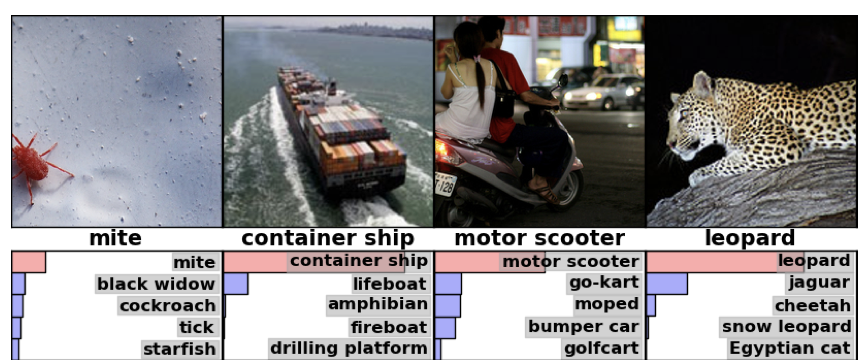
\includegraphics[width=0.8\textwidth]{ figures/intro/alexnet.png}
			\caption{Ejemplo de aplicación de \textit{AlexNet}. Imagen obtenida de~\cite{NIPS2012_4824}.}
			\label{fig.alexnet}
		\end{center}
\end{figure}
\vspace{-10pt}

Para la detección, una de las estructuras con mejores prestaciones y más utilizada, es la denominada \textit{YOLO}~\cite{Redmon2016YouOL}, cuyo ejemplo de funcionamiento se muestra en la Figura~\ref{fig.yolo}. Esta estructura destaca en la tarea de detección visual por rapidez y buen funcionamiento en tiempo real, gracias a la filosofía de buscar una única vez en la imagen. Su gran éxito ha hecho que la estructura haya ido evolucionando con el tiempo, dando lugar a distintas versiones que proporcionan diferentes prestaciones al usuario.

\vspace{10pt}
\begin{figure}[H]
		\begin{center}
			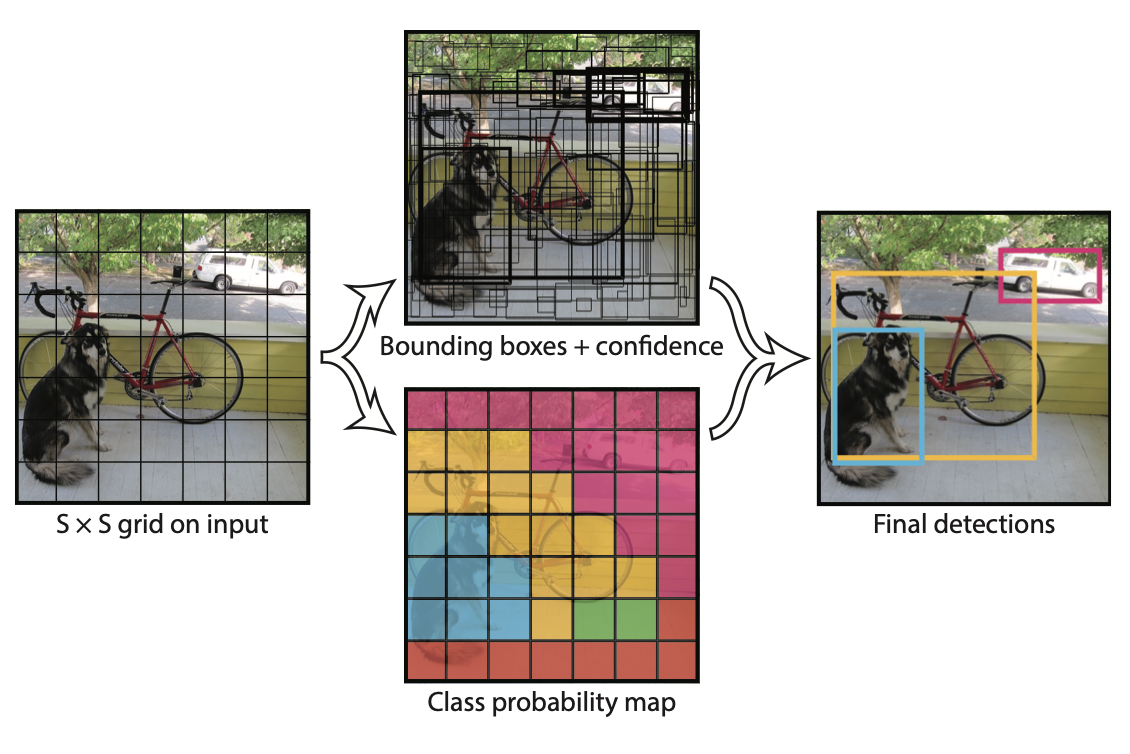
\includegraphics[width=0.7\textwidth]{ figures/intro/yolo.png}
			\caption{Ejemplo de funcionamiento de \textit{YOLO}. Imagen obtenida de~\cite{Redmon2016YouOL}.}
			\label{fig.yolo}
		\end{center}
\end{figure}
\vspace{-10pt}


Por último, existen distintos \textit{middleware} neuronales que proporcionan al desarrollador distintas herramientas para el entrenamiento y ejecución de las redes. Algunos de estos \textit{middleware} son:

\begin{itemize}
    \item \textit{Keras}
    \item \textit{Tensorflow}, desarrollado por \textit{Google}
    \item \textit{Darknet}
    \item \textit{Pytorch}, desarrollado por \textit{Facebook}
    \item \textit{Caffe}
\end{itemize}


Para la investigación de este proyecto se han considerado dos tipos de redes, recurrentes y no recurrentes, cuya principal divergencia es la persistencia del conocimiento a lo largo del tiempo. Entre ellas hay diferencias en la arquitectura de la red, y por tanto el proceso de aprendizaje. Ambos tipos se detallan a continuación.

\subsection{No recurrentes}
Las redes neuronales no recurrentes no utilizan la persistencia a lo largo del tiempo, ya que las salidas o procesamientos intermedios únicamente alimentan a la siguiente capa y no vuelven a las entradas de la propia red. Si se asemeja el funcionamiento de estas redes con la forma de pensar del ser humano, es como si cada vez que éste leyera un texto, procesase cada palabra por separado, ignorando el contexto en la que se encuentra~\cite{lstm}.\\

Este tipo de redes son las más utilizadas para abordar tareas de clasificación o detección en las que sólo es necesario procesar una imagen puntual para  extraer información de la misma. En este trabajo se plantea el uso de dos estructuras no recurrentes: el perceptrón multicapa, para las posiciones, y las redes convolucionales, para las imágenes. 

\subsubsection{Perceptrón multicapa} \label{ap.mlp}
Un \acrfull{mlp}\cite{mlp} es un conjunto de varios perceptrones que se apilan en varias capas para resolver problemas complejos. El perceptrón, o neurona, es una estructura simple  de clasificación binaria que fue propuesto por Cornell Frank Rosenblat en el año 1958. Se trata de una máquina de aprendizaje muy simple que toma una serie de entradas ponderadas por un peso y genera una salida de binaria: ``0'' ó ``1''. Sin embargo, el poder de estas estructuras se acentúa cuando se combinan varias de ellas, organizadas en distintas capas. En la Figura~\ref{fig.mlp} se muestra un ejemplo de una estructura~\acrshort{mlp}.
\vspace{5pt}
\begin{figure}[H]
	\begin{center}
		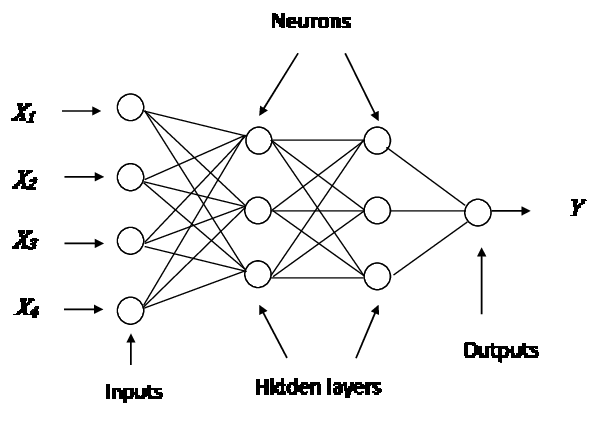
\includegraphics[width=0.58\textwidth]{ figures/intro/mlp.png}
		\caption{Estructura de perceptrón multicapa con 4 entradas, 1 salida y 2 capas ocultas. Imagen obtenida de~\cite{mlpstruct}.}
		\label{fig.mlp}
	\end{center}
\end{figure}
\vspace{-10pt}

Al tratarse de una red multicapa, ésta tiene una capa de entrada, un conjunto de capas ocultas y una capa de salida. En el \acrshort{mlp}, cada una de las neuronas de una capa envía información a las neuronas de la capa siguiente, lo que hace que la complejidad se eleve exponencialmente con el aumento de capas y de neuronas por capa oculta. Con esta estructura se pueden aproximar relaciones no lineales entre los datos de entrada y salida. 

\subsubsection{Redes convolucionales} \label{ap.cnn}
Al trabajar con imágenes éstas se deben de tratar como un conjunto de píxeles en entre los que existe una determinada correlación espacial. Las \acrfull{cnn}~\cite{cnn} son un tipo especial de \acrshort{rna} que pretende obtener correlaciones espaciales invariantes a ciertas transformaciones de la entrada. Existen \acrshort{cnn} que aplican la convolución sobre una dimensión, en un vector, sobre dos dimensiones, en una imagen, y sobre tres dimensiones, en un volumen. Para este trabajo se utilizan redes 2D, cuya estructura se representa en la Figura~\ref{fig.cnn}. El origen de este tipo de redes se sitúa en  la solución a un problema común en los \acrshort{mlp}. Este problema tiene su origen en que, en las estructuras de tipo \acrshort{mlp}, todas las capas están conectadas entre sí, obviando posibles relaciones espaciales en la imagen. 

\vspace{5pt}
\begin{figure}[H]
	\begin{center}
		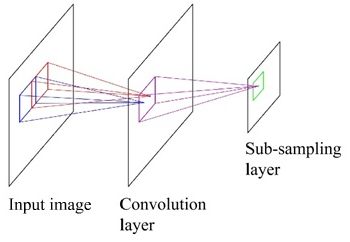
\includegraphics[width=0.5\textwidth]{ figures/intro/cnn.png}
		\caption{Estructura de \acrshort{cnn}. Imagen obtenida de~\cite{cnn}.}
		\label{fig.cnn}
	\end{center}
\end{figure}
\vspace{-10pt}

Para formar una \acrshort{cnn} se utilizan dos tipos de capas distintas conectadas entre sí. En primer lugar se emplea una capa convolucional que realiza una operación de convolución espacial sobre la imagen. Esta convolución se realiza, en cada neurona, con un filtro local cuyos pesos se modifican en durante el aprendizaje. A esta capa le sigue siempre una de submuestreo o agrupación, encargada de generar las características invariantes mediante el cálculo de estadísticas de las activaciones obtenidas a partir de un pequeño campo receptivo. Al contrario que en las \acrshort{mlp}, cada neurona en una capa oculta se conecta a un pequeño campo de la capa anterior, campo receptivo local, permitiendo mantener esa información espacial. Por otro lado, al igual que en el \acrshort{mlp}, las neuronas se organizan en varias capas consecutivas que dan lugar a distintos mapas de características. En resumen, cada mapa de características se conecta a un campo receptivo local. Además, en un mismo mapa de características se comparte el mismo parámetro de pesos, filtro o \textit{kernel}.\\

En definitiva, las \acrshort{cnn} realizan un procesamiento que trata de imitar al cortex visual del ojo humano, con el objetivo de identificar características en la entrada que permitan ``ver'' a la máquina.\\

Por último, en este trabajo no se emplean imágenes aisladas, se utilizan secuencias de vídeo que centran el elemento a procesar en un fotograma, una imagen que es tratada como un conjunto de píxeles en el que las relaciones espacio-temporales de los mismos importan.

\subsection{Recurrentes}
Las \acrfull{rnn}~\cite{lstm}, al contrario que las anteriores, sí que introducen el concepto de la persistencia en su forma de aprendizaje. Para lograr esto se introduce un bucle en la estructura que permite a los pasos siguientes de la red utilizar cierta información de los anteriores, de forma que ahora la información sí puede progresar de las siguientes capas a las anteriores, las precedentes en el flujo de datos. Para comprender mejor su funcionamiento, en la Figura~\ref{fig.rnn} se muestra un ejemplo de esta estructura, tanto de forma compacta como desenrollada.
\vspace{10pt}
\begin{figure}[H]
	\begin{center}
		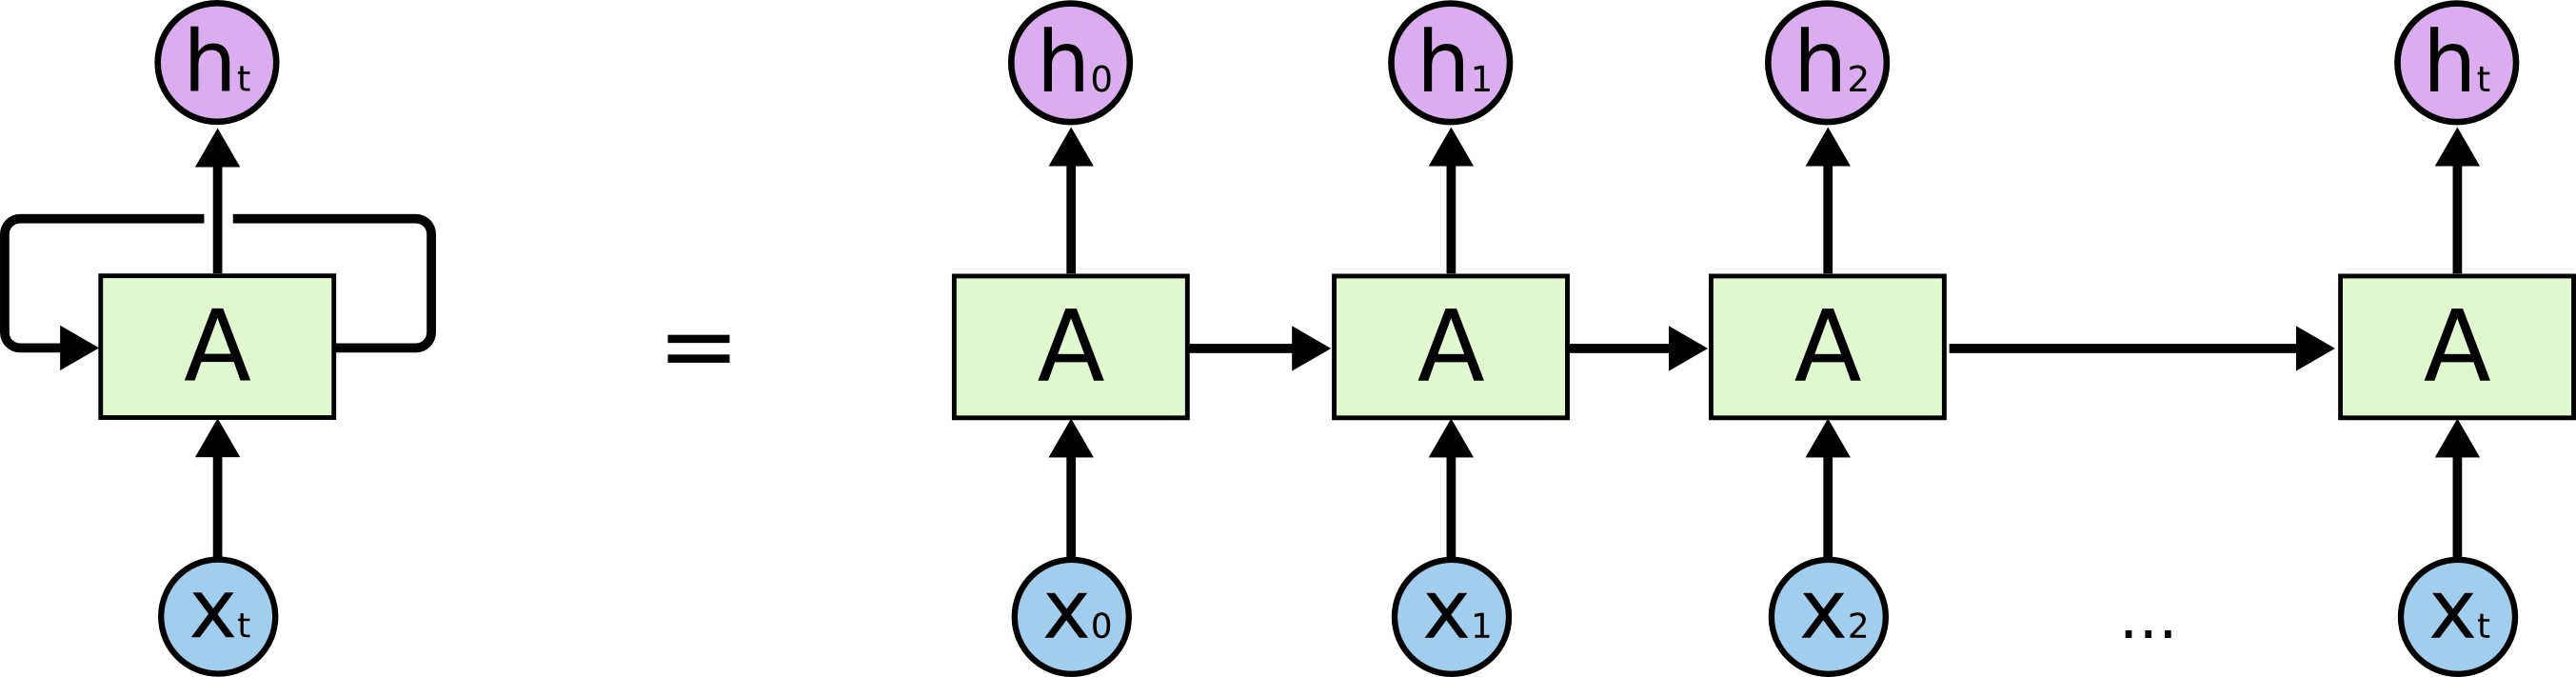
\includegraphics[width=0.65\textwidth]{ figures/intro/rnn.png}
		\caption{Estructura de RNN. Imagen obtenida de~\cite{lstm}.
		}
		\label{fig.rnn}
	\end{center}
\end{figure}
\vspace{-10pt}

Una \acrshort{rnn} puede ser vista como una misma red estática reproducida varias veces, de forma que cada copia le pasa un mensaje a la siguiente. La naturaleza de estructura en cadena hace que este tipo de redes esté íntimamente relacionado con listas y datos secuenciales, tema sobre el que versa este trabajo.

\subsubsection{Redes LSTM} \label{ap.lstm}
Las redes \acrfull{lstm}~\cite{lstm} son un tipo concreto de \acrshort{rnn} que trata de solucionar el problema de las dependencias a largo plazo. Dependiendo de la naturaleza del problema a tratar, es posible que se necesite de un contexto de mayor o menor alcance. Cuando la cantidad de características previas utilizadas no es muy grande, las \acrshort{rnn} tradicionales ofrecen buenas prestaciones. No obstante, según se amplía esta cantidad de características utilizadas, las prestaciones decrecen en consecuencia, algo que no ocurre con las \acrshort{lstm}. La estructura de este tipo de redes, mostrada en la Figura~\ref{fig.lstm}, se caracteriza por tener cuatro capas en una única celda de memoria, equivalente a las neuronas en las redes no recurrentes.

\vspace{10pt}
\begin{figure}[H]
	\begin{center}
		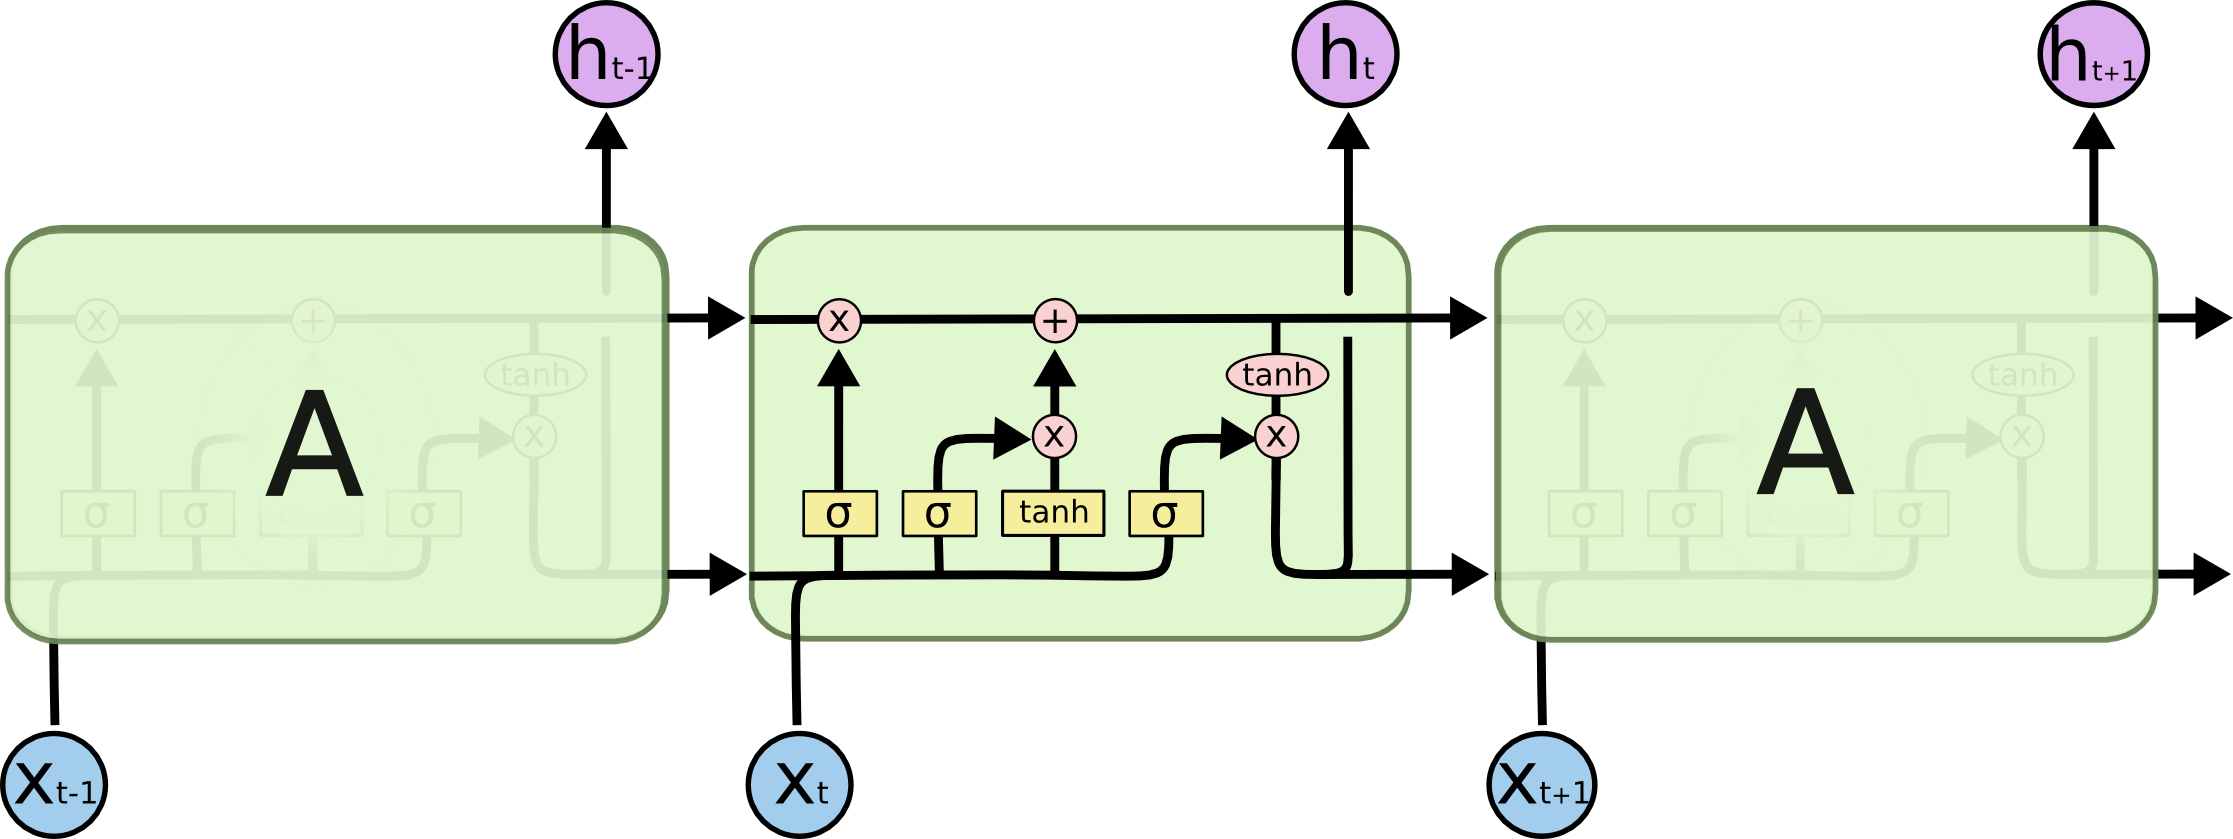
\includegraphics[width=0.7\textwidth]{ figures/intro/lstm.png}
		\caption{Estructura de LSTM. Imagen obtenida de~\cite{lstm}.
		}
		\label{fig.lstm}
	\end{center}
\end{figure}
\vspace{-10pt}

La clave de las \acrshort{lstm} se encuentra en la parte superior de la celda, su estado. Esta parte es la encargada de transportar las características de una celda a otra, con las modificaciones reguladas por tres estructuras llamadas puertas. Las puertas están compuestas por una capa sigmoidea, que genera valores entre cero y uno describiendo cuánto de cada componente de un vector de características se debe dejar pasar, seguida de una operación de multiplicación puntual. Para la modificación de los datos corren de una celda a otra se realizan cuatro pasos:

\begin{enumerate}
    \item Decidir las características antiguas a olvidar mediante la ``puerta del olvido''.
    \item Decidir las características nuevas a almacenar mediante la combinación de la ``puerta de entrada'', responsable qué valores se van a actualizar, con una capa sigmoidea que crea los nuevos valores a tomar.
    \item Actualizar las características y combinarlas en un nuevo estado que se transmitirá a la siguiente celda.
    \item Obtener la salida de la celda~(\textit{h}) como una versión filtrada del estado de la celda. Para ello se combina la ``puerta de salida'', que decide qué parte del estado de celda se considera como salida, con el propio estado de celda ponderado con una \textit{tanh} para que los valores se encuentren entre -1 y 1.
\end{enumerate}

Con este funcionamiento se consigue mantener la memoria tanto a corto plazo como a largo plazo, proporcionando buenos resultados en tareas de predicción haciendo uso de secuencias.

\subsubsection{Redes \textit(ConvLSTM)} \label{ap.convLSTM}
Las redes \textit(ConvLSTM)~\cite{DBLP:journals/corr/ShiCWYWW15} son un caso especial de las redes \acrshort{lstm} que ponen su foco en las secuencias de imágenes. La Figura~\ref{fig.convlstm} muestra la estructura de estas redes.

\vspace{10pt}
\begin{figure}[H]
	\begin{center}
		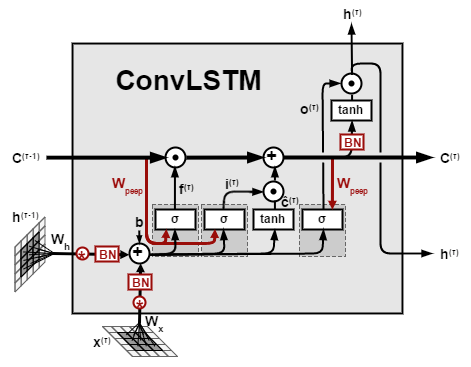
\includegraphics[width=0.7\textwidth]{ figures/intro/convLSTM.png}
		\caption{Estructura de \textit{ConvLSTM}. Imagen obtenida de~\cite{convlstm}.
		}
		\label{fig.convlstm}
	\end{center}
\end{figure}
\vspace{-10pt}

La característica principal de este tipo de redes es la capacidad de mantener las relaciones temporales, al igual que las \acrshort{lstm}, añadiendo las relaciones espaciales, propio de las \acrshort{cnn}. Para ello, se sustituyen todas las operaciones de multiplicación existentes en una celda \acrshort{lstm}, representada en la Figura~\ref{fig.lstm}, por operaciones de convolución, manteniendo las dimensiones de entrada. Este hecho consigue que esta estructura sea considerada la más idónea en tareas de predicción haciendo uso de secuencias de vídeo.

\section{Predicción con Redes Neuronales Artificiales}
En este trabajo se plantea un proceso de aprendizaje supervisado con secuencias de imágenes, es decir, de \acrshort{va}. Los algoritmos supervisados utilizados en este campo típicamente pueden abordar tareas de tres tipologías diferentes: clasificación, detección y predicción. Los dos primeros tipos abarcan la gran mayoría de soluciones actuales en el mercado. En cuanto a la predicción, actualmente se está investigando mucho y hay numerosas soluciones satisfactorias en distintos ámbitos, debido a su gran potencial.\\

\begin{figure}[H]
		\begin{center}
			\subfigure[]{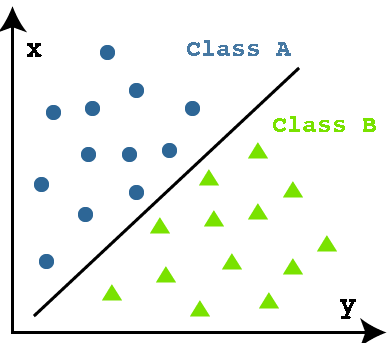
\includegraphics[width=0.25\textwidth]{ figures/intro/classification.png}} \hspace{10pt}
	        \subfigure[]{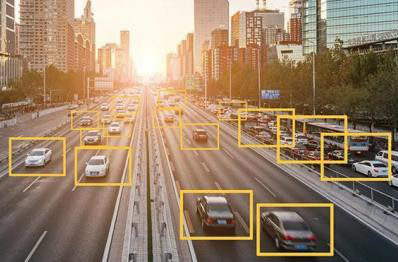
\includegraphics[width=0.3\textwidth]{ figures/intro/traffic.jpg}} \hspace{10pt}
	        \subfigure[]{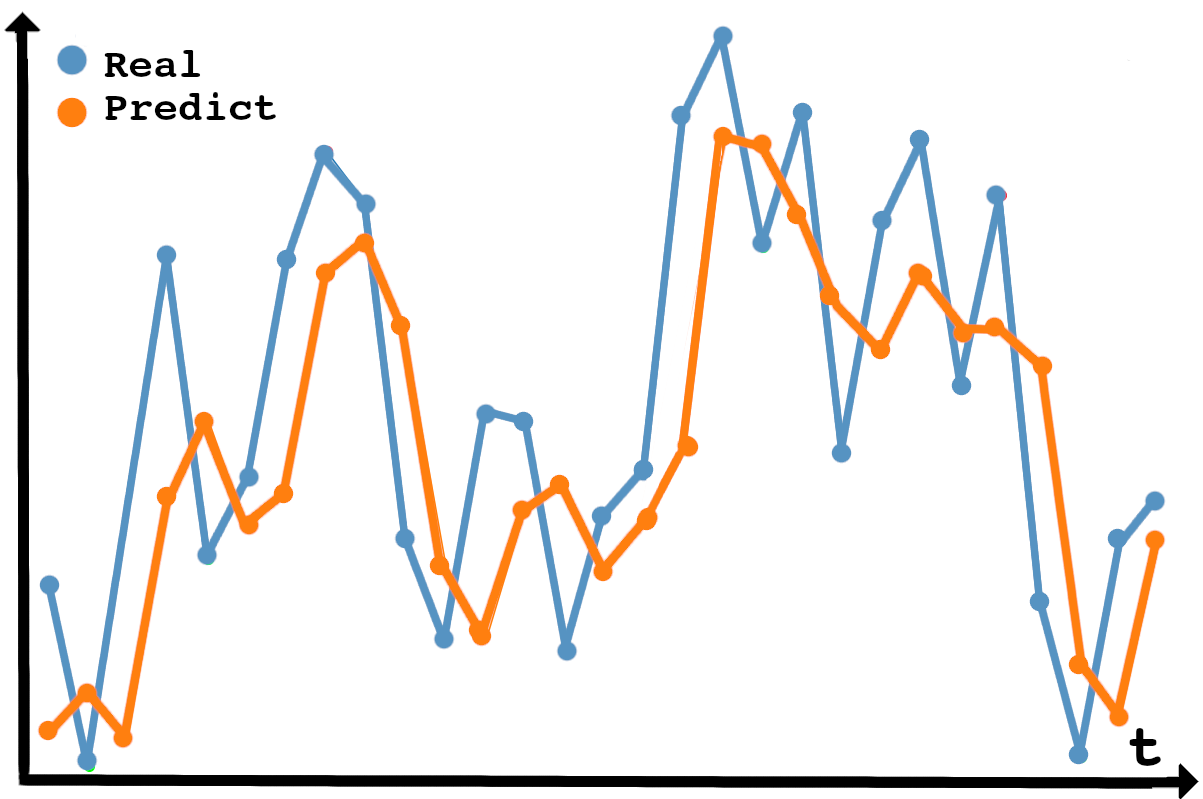
\includegraphics[width=0.35\textwidth]{ figures/intro/predict.png}}
	        \caption{Tareas de: (a)~Clasificación, (b)~Detección y (c)~Predicción.}
			\label{fig.problemas}
		\end{center}
\end{figure}
\vspace{-10pt}

En las tareas de clasificación, el objetivo principal de los algoritmos es establecer la pertenencia de un ejemplo a una clase de un conjunto previamente definido. En la detección, el algoritmo busca un patrón en la imagen y establece la posición del objeto dentro de la misma. Por último, la predicción se suele afrontar como una tarea de regresión, en el que el valor de aproximación que se obtiene a la salida no tiene ningún límite.\\

Muchos de los ejemplos de predicción actuales están enfocados a valores económicos, como la acción el Bolsa, la evolución de los precios de recursos naturales o las ventas futuras de una compañía. Todos ellos toman como entrada un conjunto de datos numéricos y su salida tiene la misma naturaleza. En la Figura~\ref{fig.trading} se presenta una de estas aplicaciones para la predicción del precio de las acciones en actividades de \textit{trading}.

\vspace{10pt}
\begin{figure}[H]
		\begin{center}
			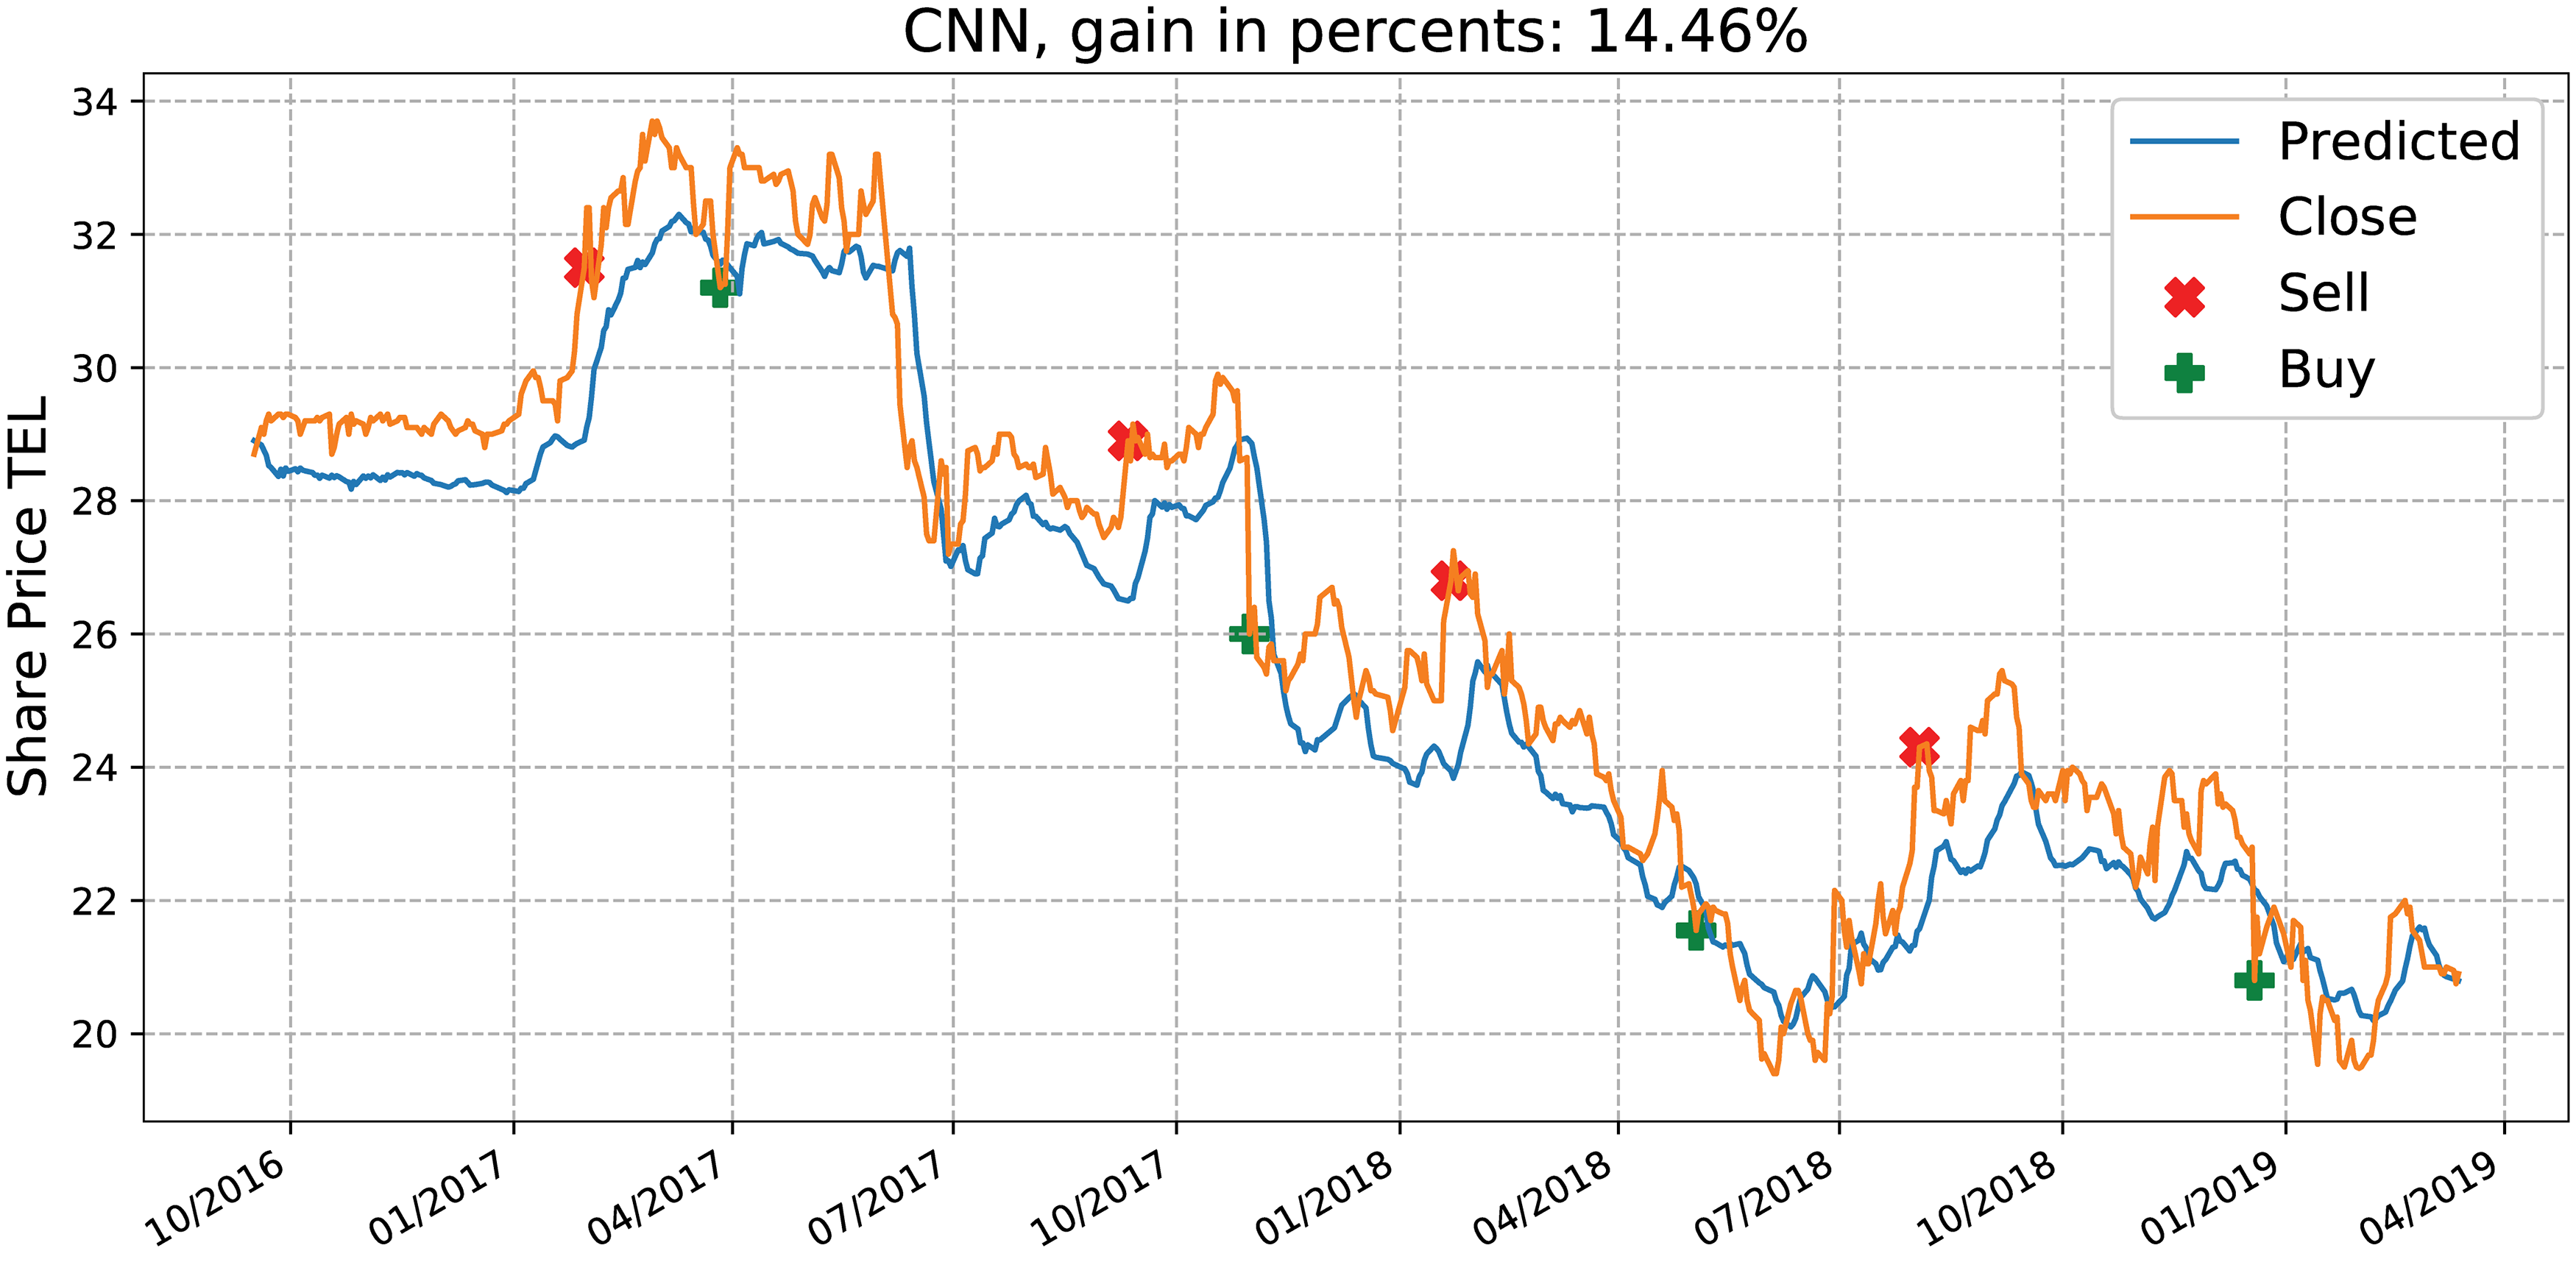
\includegraphics[width=0.8\textwidth]{ figures/intro/trading.PNG}
			\caption{Ejemplo de predicción en \textit{trading}. Imagen obtenida de~\cite{2019PLoSO..1423593S}.}
			\label{fig.trading}
		\end{center}
\end{figure}
\vspace{-10pt}

La predicción de fotogramas por una máquina es algo que puede resultar muy útil en contextos como la videovigilancia o la programación de autómatas, y que cada vez tiene mayor interés en el mundo tecnológico y, en concreto, en el campo de la Visión Artificial. En los últimos años se ha producido un gran progreso de la predicción en el ámbito de secuencias numéricas. En contraste, la tarea de predicción sobre las imágenes de un vídeo tiene aún un amplio campo de exploración.\\

Respecto al uso de secuencias de imágenes, un ejemplo de aplicación es la predicción de la acción futura en una escena, cuyo ejemplo se muestra en la Figura~\ref{fig.action}. Este tipo de aplicación puede resultar útil, por ejemplo en la mejora de la interacción entre un robot y una persona. Al analizar el movimiento de la persona frente a la cámara del robot, éste puede predecir el próximo movimiento del humano y anticiparse para ofrecer una mejor experiencia al usuario.
\vspace{10pt}
\begin{figure}[H]
	\begin{center}
		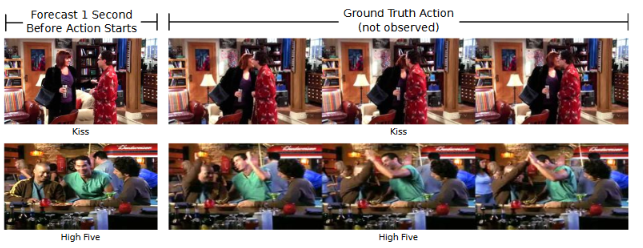
\includegraphics[width=0.85\textwidth]{ figures/intro/action.PNG}
		\caption{Predicción de acciones en secuencia de vídeo. Imagen obtenida de~\cite{unlabeledvideo}.
		}
		\label{fig.action}
	\end{center}
\end{figure}
\vspace{-10pt}
Otro ejemplo de aplicación de la predicción con secuencias de vídeo se focaliza en el ámbito de los videojuegos. Gracias a la tecnología de predicción se mejora la experiencia del jugador, mostrando una situación del juego acorde a los movimientos que éste realiza con los elementos de control~(véase la Figura~\ref{fig.game}). De esta forma se consigue que el juego siga una dinámica más fluida y se adapte al nivel del propio jugador, evitando niveles imposibles y el consecuente abandono de la partida.

\begin{figure}[H]
	\begin{center}
		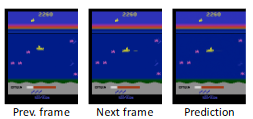
\includegraphics[width=0.65\textwidth]{ figures/intro/game.PNG}
		\caption{Predicción del fotograma en un videojuego. Imagen obtenida de~\cite{actiongames}.
		}
		\label{fig.game}
	\end{center}
\end{figure}
\vspace{-10pt}

Un último ejemplo de aplicación a la orden del día, mostrado en la Figura~\ref{fig.drive} es la asistencia a la conducción. Son muchas las situaciones que hacen que un conductor tenga que planificar sus decisiones en un corto espacio de tiempo. El procesamiento de las imágenes tomadas por el vehículo para predecir lo que puede pasar en el entorno que rodea al mismo, puede ayudar en la toma de decisiones por parte del conductor. Esta mejora en la conducción acerca, a su vez, la posibilidad de que en un futuro los vehículos no necesiten de la acción humana.
\vspace{5pt}
\begin{figure}[H]
	\begin{center}
		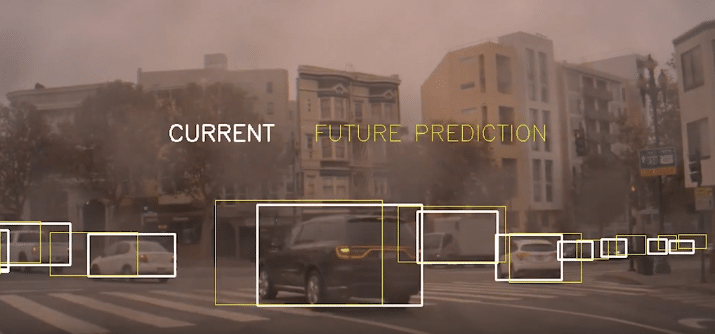
\includegraphics[width=0.7\textwidth]{ figures/intro/drive.png}
		\caption{Predicción en asistencia a la conducción. Imagen obtenida de~\cite{drive}.
		}
		\label{fig.drive}
	\end{center}
\end{figure}
\vspace{-10pt}

\section{Objetivos} \label{sec.obj}
El objetivo principal de este trabajo es diseño y el análisis de distintas redes neuronales como predictores visuales mediante el procesamiento de secuencias de vídeo. Se propone investigar las prestaciones de varias estructuras de redes neuronales con secuencias de fotogramas que muestran por diferentes dinámicas de movimiento más o menos complejas de predecir.\\

Para cumplir con el objetivo se han considerado dos tipos de imágenes: las crudas, imágenes normales que representan cada fotograma como una matriz 2D donde cada píxel tiene un valor de luminancia, y las modeladas, donde se asume que hay un único píxel blanco sobre fondo negro que se va moviendo a lo largo de la secuencia. Cada imagen modelada es un resumen de la posición (\textit{x, y}) de ese píxel activo, de modo que la secuencia de fotogramas se resume en un vector de posiciones a lo largo del tiempo.\\

El anterior objetivo general ha sido articulado en los siguientes 4 subobjetivos:
\begin{enumerate}
    \item \textbf{Desarrollo \textit{software}} del código necesario para ejecución de redes neuronales, conexión con imágenes de entrada, muestra de sus inferencias y grabación de sus estimaciones. También se programará el \textit{software} para la evaluación automáticas de varias figuras de mérito.
    \item \textbf{Creación de las bases de datos} con las que entrenar las distintas redes propuestas y  evaluar sus prestaciones. Los conjuntos se crearán bajo la premisa de un píxel activo que se mueve en la imagen siguiendo una dinámica determinada. Se programará un generador de fotogramas sintéticos.
    \item \textbf{Estudio y evaluación} de las prestaciones de varias redes no recurrentes y de varias redes recurrentes para predecir en secuencias de \textbf{imágenes modeladas}.
    \item \textbf\textbf{Estudio y evaluación} de las prestaciones de varias redes no recurrentes y de varias redes recurrentes para predecir en secuencias de \textbf{imágenes crudas}.
\end{enumerate}


\section{Metodología}

Con el propósito de alcanzar los objetivos establecidos se han utilizado una serie de herramientas y métodos que han favorecido un seguimiento fluido y dinámico de los avances en el proyecto.\\

La herramienta principal para mantener una interacción continua con los tutores ha sido el establecimiento de reuniones, generalmente semanales, en las que actualizar el trabajo realizado durante la semana, poner en común y discutir los resultados obtenidos, consultar algunas dudas y establecer los pasos a seguir durante la siguiente semana. De forma adicional, para permitir un seguimiento durante la semana a todos los miembros del grupo y dejar patentes los avances obtenidos, se ha empleado un repositorio de GitHub\footnote{\url{https://github.com/RoboticsLabURJC/2017-tfm-nuria-oyaga}} donde se dispone del código y una bitácora\footnote{\url{https://roboticslaburjc.github.io/2017-tfm-nuria-oyaga/}} en la que se presentan esos avances.\\


En cuanto a la metodología de la realización del trabajo, se ha utilizado un enfoque en espiral, como el representado en la Figura~\ref{fig.espiral}. Se definen cuatro fases principales, que son recorridas en forma de caracola: 
\begin{enumerate}
    \item Fase de planificación en la que se marcan los objetivos a alcanzar.
    \item Fase de análisis de los posibles problemas a afrontar durante el desarrollo.
    \item Fase de desarrollo, que generalmente coincide con el entrenamiento y la obtención de resultados de las distintas redes.
    \item Fase de evaluación, en la que se analizan los resultados y se toman decisiones sobre los pasos a seguir según las conclusiones.
\end{enumerate}

\begin{figure}[H]
	\begin{center}
		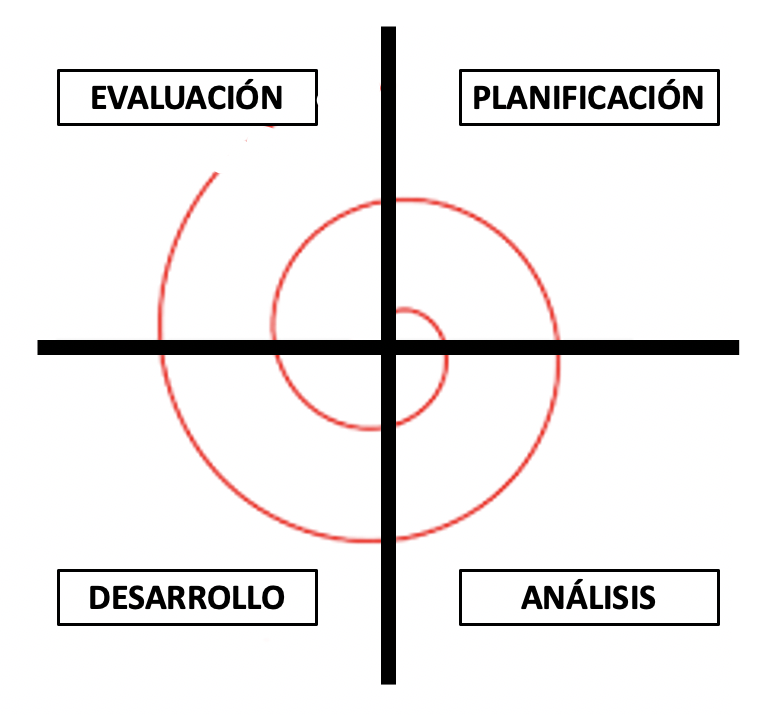
\includegraphics[width=0.5\textwidth]{ figures/intro/espiral.png}
		\caption{Enfoque en espiral.}
		\label{fig.espiral}
	\end{center}
\end{figure}
\vspace{-10pt}

Aunque no se establece un número fijo de iteraciones sobre este esquema, generalmente cada iteración coincide con el tiempo transcurrido entre reunión y reunión, aumentando el alcance del trabajo.

\section{Estructura de la memoria}
En el \textbf{Capítulo 1, Introducción,} se sitúa el trabajo en el marco actual de la tecnología, la \acrshort{ia} y la sociedad en general. Se establece el contexto de la \acrshort{va} y de la tarea de predicción, sobre la que gira este trabajo. Además, se explican las \acrshort{rna} y se describen las principales estructuras consideradas en el desarrollo. También se establecen las metas que se pretenden alcanzar con el mismo.\\

En el \textbf{Capítulo 2, Estado del arte,} se exponen algunas líneas de investigación referentes a la predicción, tanto en datos numéricos como en imágenes, que proporcionaron avances en dicho campo. Posteriormente se explica la infraestructura, tanto \textit{software} como \textit{hardware}, empleada durante el desarrollo del trabajo.\\

En el \textbf{Capítulo 3, Generación de secuencias de vídeo sintéticas,} se explican los tipos de imágenes utilizados, modeladas y crudas, las dinámicas que rigen el movimiento del píxel en la imagen durante una secuencia, y la herramienta desarrollada para la generación de los conjuntos de datos.\\

En el \textbf{Capítulo 4, Figuras de mérito y evaluación,} se presentan las métricas calculadas para la evaluación de las distintas estructuras neuronales y la comparación entre ellas. Además, se describe la metodología de evaluación desarrollada y la forma de presentar los resultados obtenidos.\\

En el \textbf{Capítulo 5, Predicción con imágenes modeladas,} se exponen todos los experimentos realizados con imágenes modeladas y las diferentes dinámicas, mostrando sus resultados y extrayendo conclusiones sobre los mismos.\\

En el \textbf{Capítulo 6, Predicción con imágenes crudas,} se presentan todos los experimentos realizados con imágenes crudas y las distintas dinámicas,  mostrando sus resultados y extrayendo conclusiones sobre los mismos.\\

Por último, el \textbf{Capítulo 7, Conclusiones,} resume las conclusiones obtenidas en el trabajo y establece un posible plan de actuación futuro para continuar con la investigación en el tema abordado.

